%%%%%%%%%%%%%%%%%%%%%%%%%%%%%%%%%%%%%%%%%%%%%%%%%%%%%%%%%%%%%%%%%%%%%%%%%%%%%%%%%%
\begin{frame}[fragile]\frametitle{}
\begin{center}
{\Large Predictive Analytics}


% {\tiny (Ref: The most under-taught skill in machine learning - George Seif )}
\end{center}


\end{frame}

%%%%%%%%%%%%%%%%%%%%%%%%%%%%%%%%%%%%%%%%%%%%%%%%%%%%%%%%%%%%%%%%%%%%%%%%%%%%%%%%%%
\begin{frame}\frametitle{The Story}
Heard of ``Netflix''?
\begin{itemize}
\item Subscription-based DVD rental model and streaming service
\item Heavily use reccomendations/suggestuibs to users. 3/4th of revenues.
\item More if/once you do better recommendations.
\item Kaggle Competition: crowdsourced model development by sponsoring a contest with a \$1 million prize
\item Algorithm had to improve upon Netflix’s results by 10\%. 
\end{itemize}

{\tiny (Ref: Our Favorite Analytics Stories by JULIE GRISANTI )}

\end{frame}

%%%%%%%%%%%%%%%%%%%%%%%%%%%%%%%%%%%%%%%%%%%%%%%%%%%%%%%%%%%%%%%%%%%%%%%%%%%%%%%%%%
\begin{frame}\frametitle{The Story}
Solution!!!
\begin{itemize}
\item Took about three years, but eventually two teams were able to break the 10\% mark
\item Trend emerged: no individual team could quite make the 10\% mark, 
so teams started to merge into mega-teams, 
and also merged their individual models into ensembles of models; 
\item Result: these ensembles performed better than any of the individual models. 

\end{itemize}

{\tiny (Ref: Our Favorite Analytics Stories by JULIE GRISANTI )}

\end{frame}

%%%%%%%%%%%%%%%%%%%%%%%%%%%%%%%%%%%%%%%%%%%%%%%%%%%%%%%%%%%%%%%%%%%%%%%%%%%%%%%%%%
\begin{frame}\frametitle{The Story}
Heard of Cambridge Analytica?
\begin{itemize}
\item Barack Obama’s presidential campaigns were notable as the first to heavily rely on advanced analytics to target voters.
\item Used many data sources to micro-target individual voters. 
\item A score was calculated for each potential voter across two dimensions: who is likely to vote, and who is likely to vote for Obama. 
\item Armed with this nuanced information, canvassers knew exactly whom they should be contacting, and could personalize their messages for each individual. 
\item Donald Trump as well as Indian Political parties are using Predictive Analytics heavily (less are going to Astrologgers?)
\end{itemize}

{\tiny (Ref: Our Favorite Analytics Stories by JULIE GRISANTI )}

\end{frame}

%%%%%%%%%%%%%%%%%%%%%%%%%%%%%%%%%%%%%%%%%%%%%%%%%%%%%%%%%%%%%%%%%%%%%%%%%%%%%%%%%%
\begin{frame}[fragile]\frametitle{}
\begin{center}
{\Large What is Analytics?}
\end{center}
\end{frame}

%%%%%%%%%%%%%%%%%%%%%%%%%%%%%%%%%%%%%%%%%%%%%%%%%%%%%%%%%%%%%%%%%%%%%%%%%%%%%%%%%%
\begin{frame}\frametitle{What is Analytics?}

\begin{center}
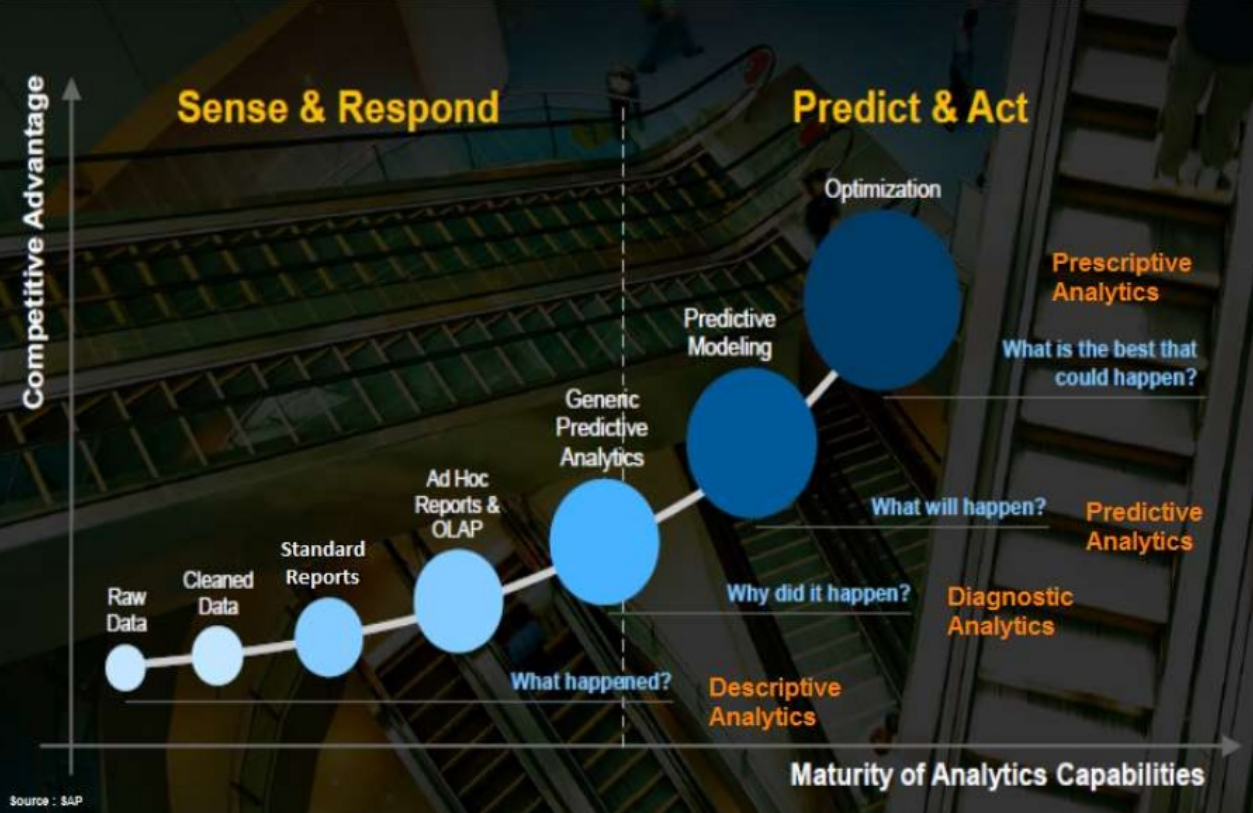
\includegraphics[width=\linewidth]{predanat3}
\end{center}

{\tiny (Ref: Predictive Analytics - An Overview - Machine Pulse )}

\end{frame}

%%%%%%%%%%%%%%%%%%%%%%%%%%%%%%%%%%%%%%%%%%%%%%%%%%%%%%%%%%%%%%%%%%%%%%%%%%%%%%%%%%
\begin{frame}\frametitle{Evolution of Data Analytics}

\begin{center}
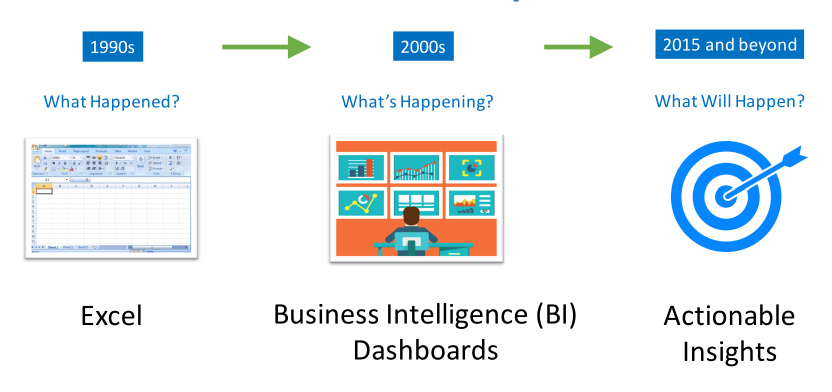
\includegraphics[width=\linewidth]{predanat16}
\end{center}

{\tiny (Ref: Predictive Analytics - Big	Data	\&	Artificial	Intelligence - October 2016 )}

\end{frame}

%%%%%%%%%%%%%%%%%%%%%%%%%%%%%%%%%%%%%%%%%%%%%%%%%%%%%%%%%%%%%%%%%%%%%%%%%%%%%%%%%%
\begin{frame}\frametitle{What is Predictive Analytics?}

\begin{itemize}
\item Using historical data, machine learning, and artificial intelligence to predict what will happen in the future.  
\item This historical data is fed into a mathematical model that considers key trends and patterns in the data. 
\item The model is then applied to current data to predict what will happen next.
\end{itemize}

\begin{center}
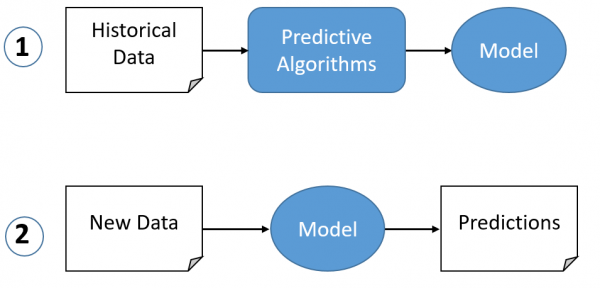
\includegraphics[width=0.6\linewidth]{predanat1}
\end{center}


{\tiny (Ref: What Is Predictive Analytics? BY SRIRAM PARTHASARATHY )}

\end{frame}

%%%%%%%%%%%%%%%%%%%%%%%%%%%%%%%%%%%%%%%%%%%%%%%%%%%%%%%%%%%%%%%%%%%%%%%%%%%%%%%%%%
\begin{frame}\frametitle{What is Predictive Analytics?}

\begin{itemize}
\item Identifying cause-effect relationships across the variables from the historical data.

\item Discovering hidden insights and patterns with the help of data mining
techniques
\item Apply observed patterns to unknowns in the Past, Present or Future.
\end{itemize}


{\tiny (Ref: Predictive Analytics - An Overview - Machine Pulse )}

\end{frame}

%%%%%%%%%%%%%%%%%%%%%%%%%%%%%%%%%%%%%%%%%%%%%%%%%%%%%%%%%%%%%%%%%%%%%%%%%%%%%%%%%%
\begin{frame}\frametitle{Why to use?}
\begin{itemize}
\item Businesses are getting more complex
\item Too much data and too many variables for a human to analyze
\item Traditional analytics or statistical methods fail due to complex non-linear and multi variable combination.
\end{itemize}
\end{frame}


%%%%%%%%%%%%%%%%%%%%%%%%%%%%%%%%%%%%%%%%%%%%%%%%%%%%%%%%%%%%%%%%%%%%%%%%%%%%%%%%%%
\begin{frame}\frametitle{Where to use?}
Help companies—and business applications:
\begin{itemize}
\item Suggests actions that can affect positive operational changes.
\item Foresees if a change will help them reduce risks, improve operations, and/or increase revenue.
\item Answers the question,``What is most likely to happen based on my current data, and what can I do to change that outcome?''
\end{itemize}
\end{frame}

%%%%%%%%%%%%%%%%%%%%%%%%%%%%%%%%%%%%%%%%%%%%%%%%%%%%%%%%%%%%%%%%%%%%%%%%%%%%%%%%%%
\begin{frame}[fragile]\frametitle{}
\begin{center}
{\Large Business Applications}
\end{center}
\end{frame}


%%%%%%%%%%%%%%%%%%%%%%%%%%%%%%%%%%%%%%%%%%%%%%%%%%%%%%%%%%%%%%%%%%%%%%%%%%%%%%%%%%
\begin{frame}\frametitle{Business Applications}

\begin{center}
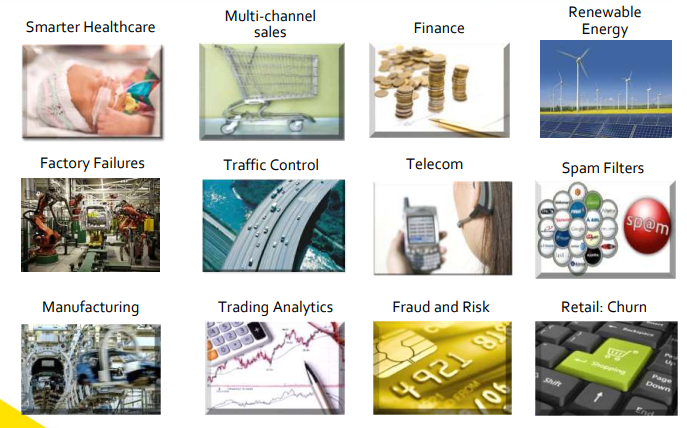
\includegraphics[width=\linewidth]{predanat5}
\end{center}

{\tiny (Ref: Predictive Analytics - An Overview - Machine Pulse )}

\end{frame}

%%%%%%%%%%%%%%%%%%%%%%%%%%%%%%%%%%%%%%%%%%%%%%%%%%%%%%%%%%%%%%%%%%%%%%%%%%%%%%%%%%
\begin{frame}\frametitle{Business Applications}
\begin{itemize}
\item Supply Chain:
Simulate and optimize supply chain flows to reduce inventory.
\item  Customer Profiling:
Identify high valued customers and retain their loyalty.
\item  Pricing:
Identify the optimal price which will increase net profit.
\item Human Resources:
Best Employees selection for particular tasks at optimal
compensation. Employee churn retention.

\end{itemize}
\end{frame}

%%%%%%%%%%%%%%%%%%%%%%%%%%%%%%%%%%%%%%%%%%%%%%%%%%%%%%%%%%%%%%%%%%%%%%%%%%%%%%%%%%
\begin{frame}\frametitle{Business Applications}
\begin{itemize}
\item Renewable Energy:
Energy forecasting, electricity price forecasting, Predictive
Maintenance, Operational cost minimization.
\item Financial Services:
Approval of credit cards/ loan applications based on credit scoring
models, Options pricing, Risk analysis etc.
\item E-Commerce:
Identify cross-sell and upsell opportunities, increase transactions
size, maximize campaign's response based CRM data.
\end{itemize}
\end{frame}

%%%%%%%%%%%%%%%%%%%%%%%%%%%%%%%%%%%%%%%%%%%%%%%%%%%%%%%%%%%%%%%%%%%%%%%%%%%%%%%%%%
\begin{frame}\frametitle{Business Applications}
\begin{itemize}
\item Product Quality Control:
Detect product quality issues in advance and prevent them.
\item  Revenue Performance:
Identify key drivers of revenue generation and optimization of
revenue.
\item  Fraud and Crime Detection:
Detect fraud , criminal activity, insurance claims, tax evasion and
credit card frauds.
\item HealthCare:
Identify prevalence of particular disease to a patient based health
conditions.

\end{itemize}
\end{frame}


%%%%%%%%%%%%%%%%%%%%%%%%%%%%%%%%%%%%%%%%%%%%%%%%%%%%%%%%%%%%%%%%%%%%%%%%%%%%%%%%%%
\begin{frame}[fragile]\frametitle{}
\begin{center}
{\Large Usecase}
\end{center}
\end{frame}



%%%%%%%%%%%%%%%%%%%%%%%%%%%%%%%%%%%%%%%%%%%%%%%%%%%%%%%%%%%%%%%%%%%%%%%%%%%%%%%%%%
\begin{frame}\frametitle{Real World Examples}
Applications in Business Intelligence:
\begin{itemize}
\item Io improve everyday business operations
\item To achieve a competitive differentiation
\end{itemize}

Few detailed use-cases \ldots
\end{frame}

%%%%%%%%%%%%%%%%%%%%%%%%%%%%%%%%%%%%%%%%%%%%%%%%%%%%%%%%%%%%%%%%%%%%%%%%%%%%%%%%%%
\begin{frame}\frametitle{Identify customers}
\ldots that are likely to abandon a service or product. E.g Yoga class

\begin{itemize}
\item Based on past data, the system may identify that `Rahul' will most likely not renew her membership.
\item How?
\item Suggest an incentive that is likely to get him to renew.
\item In this example, predictive analytics can be used in real time to remedy customer churn before it takes place.
\item Similar example: Job churn.
\end{itemize}

\end{frame}

%%%%%%%%%%%%%%%%%%%%%%%%%%%%%%%%%%%%%%%%%%%%%%%%%%%%%%%%%%%%%%%%%%%%%%%%%%%%%%%%%%
\begin{frame}\frametitle{Send marketing offers}
\ldots to customers who are most likely to buy.

\begin{itemize}
\item If your business only has a Rs 50,000 budget for marketing campaign and you have three lakh  customers, you obviously can’t extend a 10 percent discount to each customer. 
\item Predictive analytics and business intelligence can help forecast the customers who have the highest probability of buying your product, 
\item then send the discount coupon to only those people to optimize revenue.
\end{itemize}

\end{frame}

%%%%%%%%%%%%%%%%%%%%%%%%%%%%%%%%%%%%%%%%%%%%%%%%%%%%%%%%%%%%%%%%%%%%%%%%%%%%%%%%%%
\begin{frame}[fragile]\frametitle{}
\begin{center}
{\Large The Process}
\end{center}
\end{frame}



%%%%%%%%%%%%%%%%%%%%%%%%%%%%%%%%%%%%%%%%%%%%%%%%%%%%%%%%%%%%%%%%%%%%%%%%%%%%%%%%%%
\begin{frame}\frametitle{How Does Predictive Analytics Work?}
First, 
\begin{itemize}
\item Identify what you want to know based on past data.
\item What questions do you want to answer? 
\item What are some of the important business decisions you’ll make with the insight? 
\end{itemize}
Knowing this is a crucial first step to applying predictive analysis
\end{frame}

%%%%%%%%%%%%%%%%%%%%%%%%%%%%%%%%%%%%%%%%%%%%%%%%%%%%%%%%%%%%%%%%%%%%%%%%%%%%%%%%%%
\begin{frame}\frametitle{How Does Predictive Analytics Work?}
Next, 
\begin{itemize}
\item Consider if you have the data to answer those questions. 
\item Is your operational system capturing the needed data? 
\item How clean is it? 
\item How far in the past do you have this data, and is that enough to learn any predictive patterns?
\end{itemize}

\end{frame}

%%%%%%%%%%%%%%%%%%%%%%%%%%%%%%%%%%%%%%%%%%%%%%%%%%%%%%%%%%%%%%%%%%%%%%%%%%%%%%%%%%
\begin{frame}\frametitle{How Does Predictive Analytics Work?}
Next, 
\begin{itemize}
\item Train the system to learn from your data and can predict outcomes. 
\item When building your predictive analytics model, you’ll have to start by training the system to learn from data. 
\item It should eventually be able to identify patterns and/or trends about your customers and their behaviors. 
\item You could also run one or more algorithms and pick the one that works best for your data, or you could opt to pick an ensemble of these algorithms.
\end{itemize}

\end{frame}

%%%%%%%%%%%%%%%%%%%%%%%%%%%%%%%%%%%%%%%%%%%%%%%%%%%%%%%%%%%%%%%%%%%%%%%%%%%%%%%%%%
\begin{frame}\frametitle{How Does Predictive Analytics Work?}
Finally, 
\begin{itemize}
\item Use the insights and predictions to act on these decisions.
\item These predictive insights can be embedded into your Line of Business applications for everyone in your organization to use.
\end{itemize}

\end{frame}

%%%%%%%%%%%%%%%%%%%%%%%%%%%%%%%%%%%%%%%%%%%%%%%%%%%%%%%%%%%%%%%%%%%%%%%%%%%%%%%%%%
\begin{frame}\frametitle{System Architecture}

\begin{center}
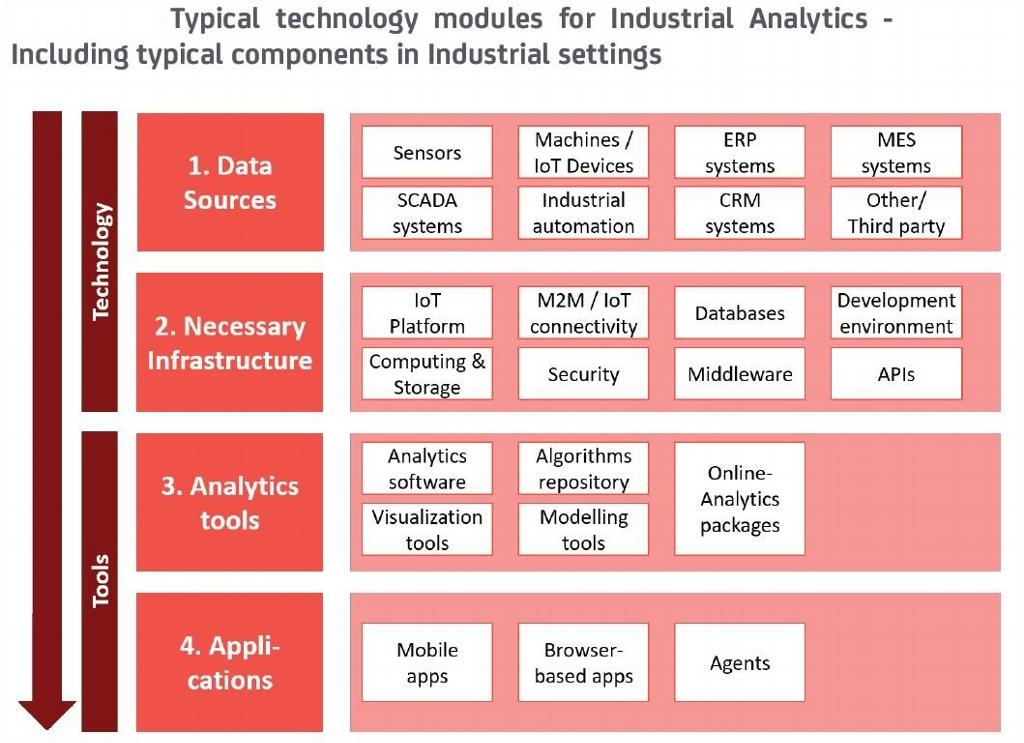
\includegraphics[width=\linewidth]{predanat21}
\end{center}

% {\tiny (Ref: Predictive Analytics - Big	Data	\&	Artificial	Intelligence - October 2016 )}

\end{frame}



%%%%%%%%%%%%%%%%%%%%%%%%%%%%%%%%%%%%%%%%%%%%%%%%%%%%%%%%%%%%%%%%%%%%%%%%%%%%%%%%%%
\begin{frame}\frametitle{The	Process of Predictive Analytics}

\begin{center}
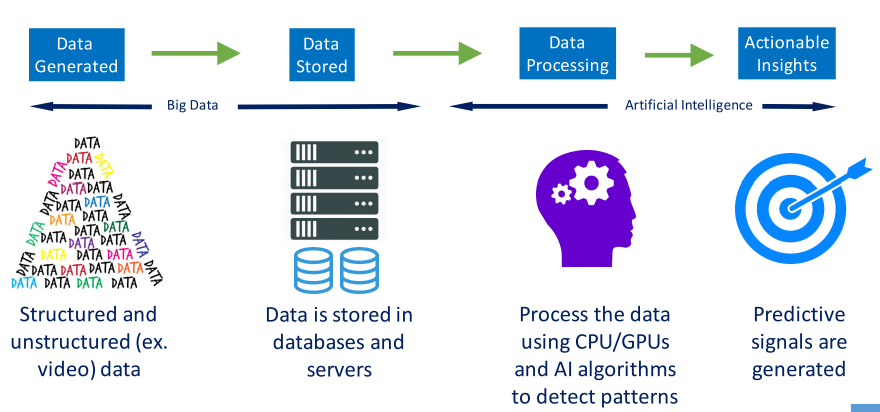
\includegraphics[width=\linewidth]{predanat17}
\end{center}

{\tiny (Ref: Predictive Analytics - Big	Data	\&	Artificial	Intelligence - October 2016 )}

\end{frame}


%%%%%%%%%%%%%%%%%%%%%%%%%%%%%%%%%%%%%%%%%%%%%%%%%%%%%%%%%%%%%%%%%%%%%%%%%%%%%%%%%%
\begin{frame}[fragile]\frametitle{}
\begin{center}
{\Large Data}
\end{center}
\end{frame}

%%%%%%%%%%%%%%%%%%%%%%%%%%%%%%%%%%%%%%%%%%%%%%%%%%%%%%%%%%%%%%%%%%%%%%%%%%%%%%%%%%
\begin{frame}\frametitle{Most Important}
Experience/Data
\begin{itemize}
\item ``Data is the new oil''. - European Consumer Commissioner Meglena Kuneva
\item ``The only source of knowledge is experience.'' - Albert Einstein
\item ``In God we trust. All others must bring data.'' - William Edwards Deming (a business professor famous for work in manufacturing)
\end{itemize}

\end{frame}

%%%%%%%%%%%%%%%%%%%%%%%%%%%%%%%%%%%%%%%%%%%%%%%%%%%%%%%%%%%%%%%%%%%%%%%%%%%%%%%%%%
\begin{frame}\frametitle{Data}
\begin{itemize}
\item As data piles up, we have ourselves a genuine gold rush. 
\item But data isn't the gold. 
\item Data in its raw form is boring crud. 
\item The gold is what's discovered therein.
\end{itemize}

\end{frame}

%%%%%%%%%%%%%%%%%%%%%%%%%%%%%%%%%%%%%%%%%%%%%%%%%%%%%%%%%%%%%%%%%%%%%%%%%%%%%%%%%%
\begin{frame}\frametitle{How	Did	We	Get	Here?}

\begin{center}
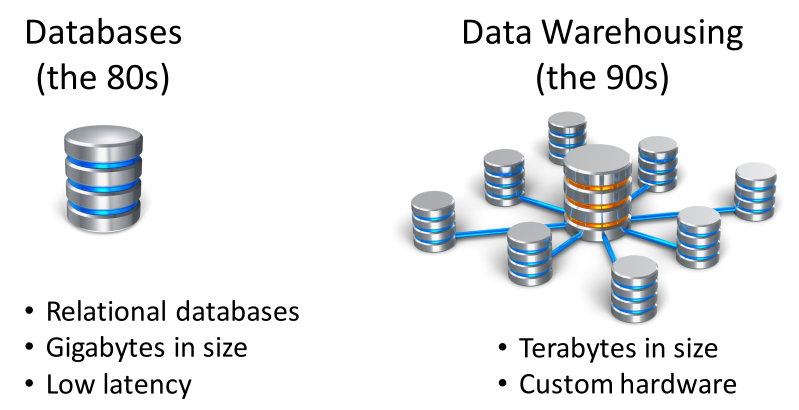
\includegraphics[width=\linewidth]{predanat18}
\end{center}

{\tiny (Ref: Predictive Analytics - Big	Data	\&	Artificial	Intelligence - October 2016 )}

\end{frame}

%%%%%%%%%%%%%%%%%%%%%%%%%%%%%%%%%%%%%%%%%%%%%%%%%%%%%%%%%%%%%%%%%%%%%%%%%%%%%%%%%%
\begin{frame}\frametitle{Today,	it's	Big	Data}

\begin{center}
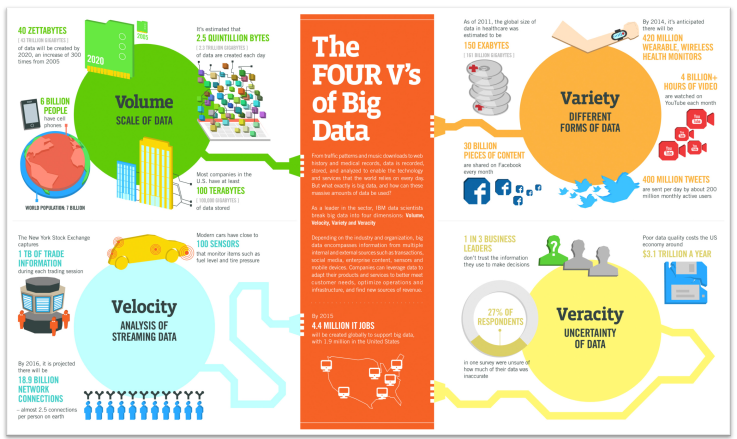
\includegraphics[width=\linewidth]{predanat19}
\end{center}

{\tiny (Ref: Predictive Analytics - Big	Data	\&	Artificial	Intelligence - October 2016 )}

\end{frame}


% %%%%%%%%%%%%%%%%%%%%%%%%%%%%%%%%%%%%%%%%%%%%%%%%%%%%%%%%%%%%%%%%%%%%%%%%%%%%%%%%%%
% \begin{frame}\frametitle{Data Processing}

% \begin{center}
% 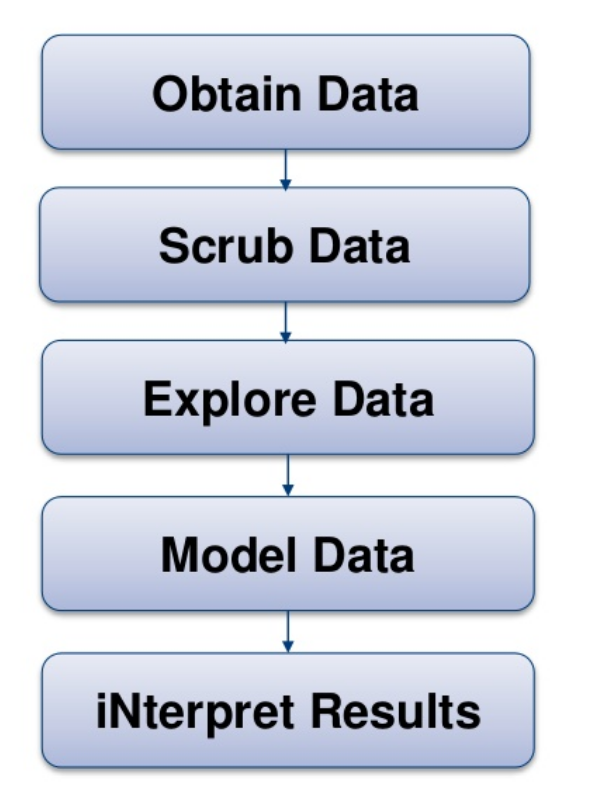
\includegraphics[width=0.4\linewidth]{predanat4}
% \end{center}

% {\tiny (Ref: Predictive Analytics - Eric Siegel )}

% \end{frame}

% %%%%%%%%%%%%%%%%%%%%%%%%%%%%%%%%%%%%%%%%%%%%%%%%%%%%%%%%%%%%%%%%%%%%%%%%%%%%%%%%%%
% \begin{frame}\frametitle{Preparing Data}

% \begin{center}
% 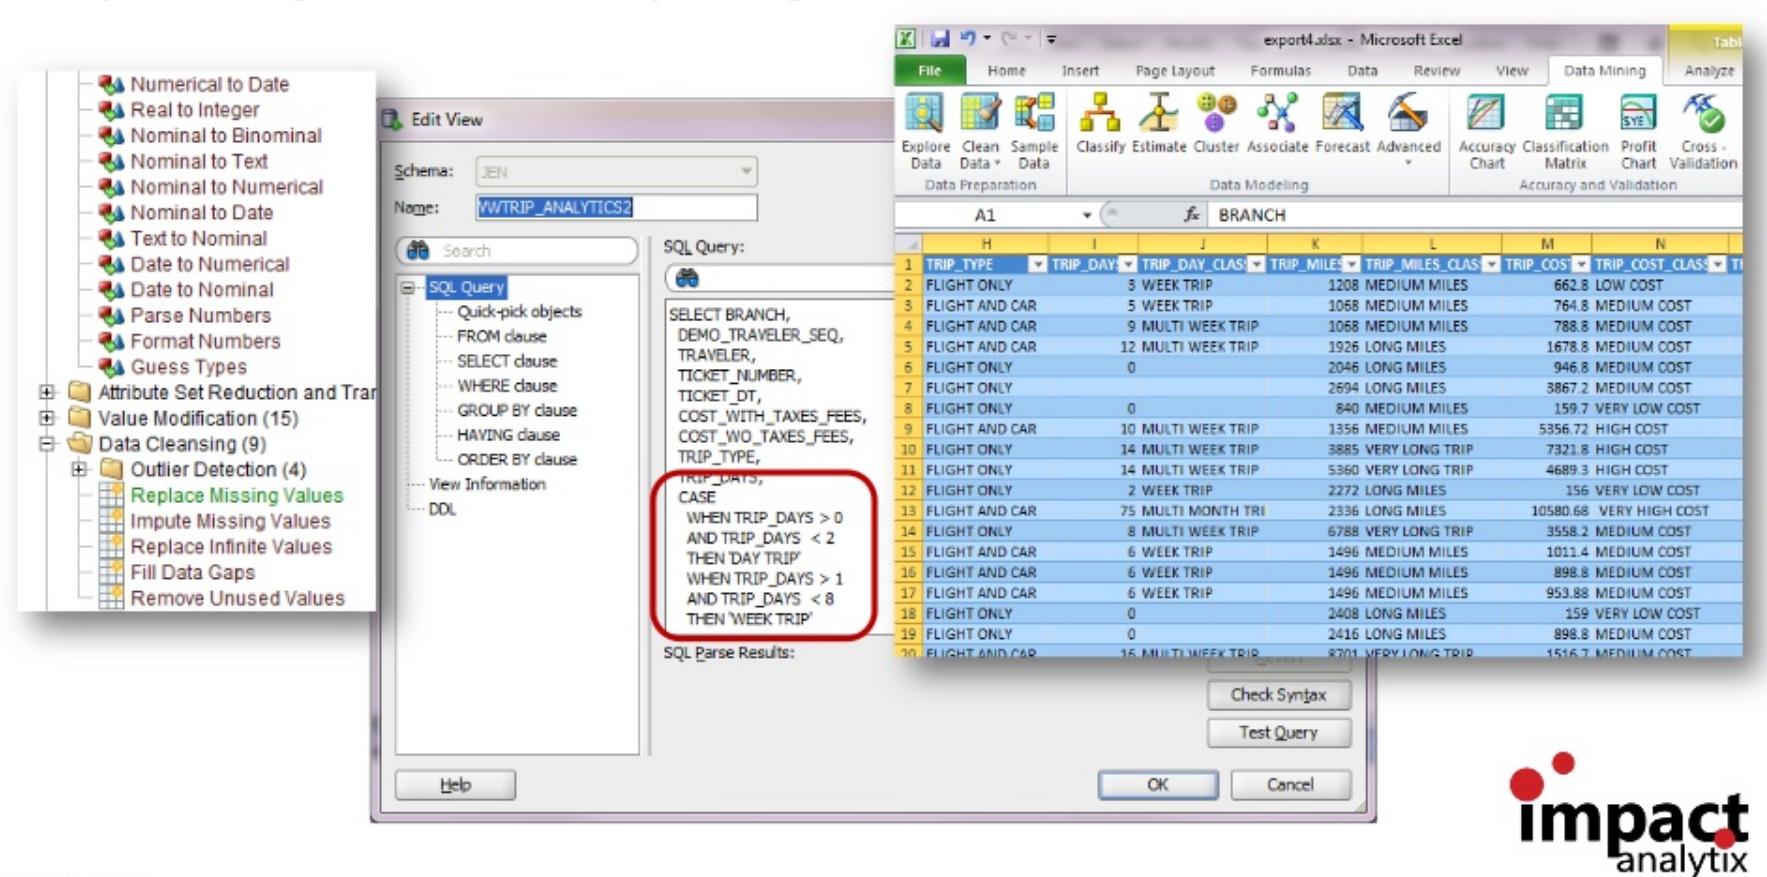
\includegraphics[width=\linewidth]{predanat7}
% \end{center}

% {\tiny (Ref: Practical Predictive Analytics - Jen Underwood )}

% \end{frame}

%%%%%%%%%%%%%%%%%%%%%%%%%%%%%%%%%%%%%%%%%%%%%%%%%%%%%%%%%%%%%%%%%%%%%%%%%%%%%%%%%%
\begin{frame}[fragile]\frametitle{}
\begin{center}
{\Large The Big Picture}
\end{center}
\end{frame}


%%%%%%%%%%%%%%%%%%%%%%%%%%%%%%%%%%%%%%%%%%%%%%%%%%%%%%%%%%%%%%%%%%%%%%%%%%%%%%%%%%
\begin{frame}\frametitle{Artificial	Intelligence	(AI)}

\begin{center}
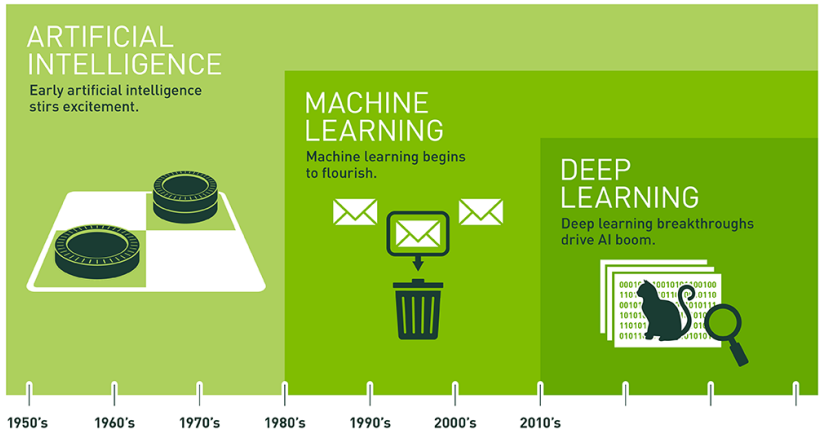
\includegraphics[width=\linewidth]{predanat20}
\end{center}

{\tiny (Ref: Predictive Analytics - Big	Data	\&	Artificial	Intelligence - October 2016 )}

\end{frame}


%%%%%%%%%%%%%%%%%%%%%%%%%%%%%%%%%%%%%%%%%%%%%%%%%%%%%%%%%%%%%%%%%%%%%%%%%%%%%%%%%%
\begin{frame}\frametitle{Machine Learning}

\begin{center}
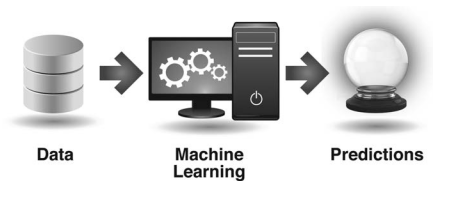
\includegraphics[width=\linewidth]{predanat2}
\end{center}

{\tiny (Ref: Predictive Analytics - Eric Siegel )}

\end{frame}

%%%%%%%%%%%%%%%%%%%%%%%%%%%%%%%%%%%%%%%%%%%%%%%%%%%%%%%%%%%%%%%%%%%%%%%%%%%%%%%%%%
\begin{frame}\frametitle{When	To	Use	Machine	Learning?}

\begin{itemize}
\item A	pattern	exists
\item We	cannot	pin	down	the	pattern	
mathematically
\item We	have	data	and	hopefully	lots	of	
data
\end{itemize}

\end{frame}

%%%%%%%%%%%%%%%%%%%%%%%%%%%%%%%%%%%%%%%%%%%%%%%%%%%%%%%%%%%%%%%%%%%%%%%%%%%%%%%%%%
\begin{frame}\frametitle{Machine Learning Methods}

\begin{itemize}
\item Regression: Predicting output variable using its cause-effect relationship with
input variables. OLS Regression, GLM, Random forests, ANN etc.
\item Classification: Predicting the item class. Decision Tree, Logistic Regression, ANN,
SVM, Naive Bayes classifier etc.
\item Time Series Forecasting: Predicting future time events given past history. AR, MA, ARIMA,
Triple Exponential Smoothing, Holt-Winters etc.
\item Clustering:
Finding natural groups or clusters in the data. K-means, Hierarchical, Spectral, Density based EM algorithm Clustering etc
\end{itemize}

\end{frame}


%%%%%%%%%%%%%%%%%%%%%%%%%%%%%%%%%%%%%%%%%%%%%%%%%%%%%%%%%%%%%%%%%%%%%%%%%%%%%%%%%%
\begin{frame}\frametitle{Evaluating Predictive Models}

\begin{itemize}
\item Scoring by Mean Squared Error or Accuracy
\item True/False positive/negatives
\item Over-fitting Under-fitting
\end{itemize}

\end{frame}

%%%%%%%%%%%%%%%%%%%%%%%%%%%%%%%%%%%%%%%%%%%%%%%%%%%%%%%%%%%%%%%%%%%%%%%%%%%%%%%%%%
\begin{frame}[fragile]\frametitle{}
\begin{center}
{\Large Tools}
\end{center}
\end{frame}


%%%%%%%%%%%%%%%%%%%%%%%%%%%%%%%%%%%%%%%%%%%%%%%%%%%%%%%%%%%%%%%%%%%%%%%%%%%%%%%%%%
\begin{frame}\frametitle{Predictive Analytics Tools in Market}

\begin{center}
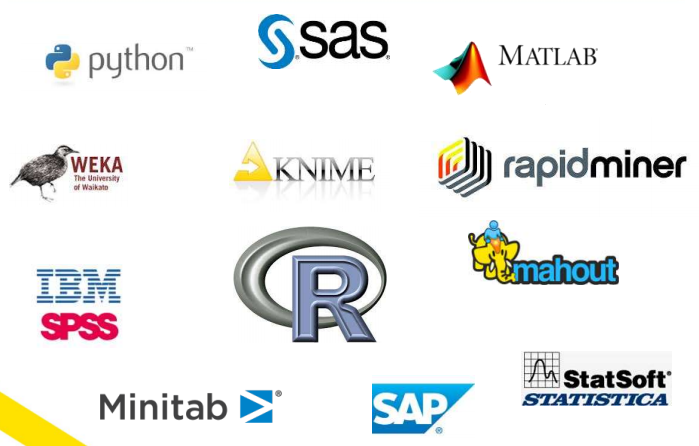
\includegraphics[width=\linewidth]{predanat6}
\end{center}

{\tiny (Ref: Predictive Analytics - An Overview - Machine Pulse )}


\end{frame}

%%%%%%%%%%%%%%%%%%%%%%%%%%%%%%%%%%%%%%%%%%%%%%%%%%%%%%%%%%%%%%%%%%%%%%%%%%%%%%%%%%
\begin{frame}\frametitle{Rapid Miner}

\begin{center}
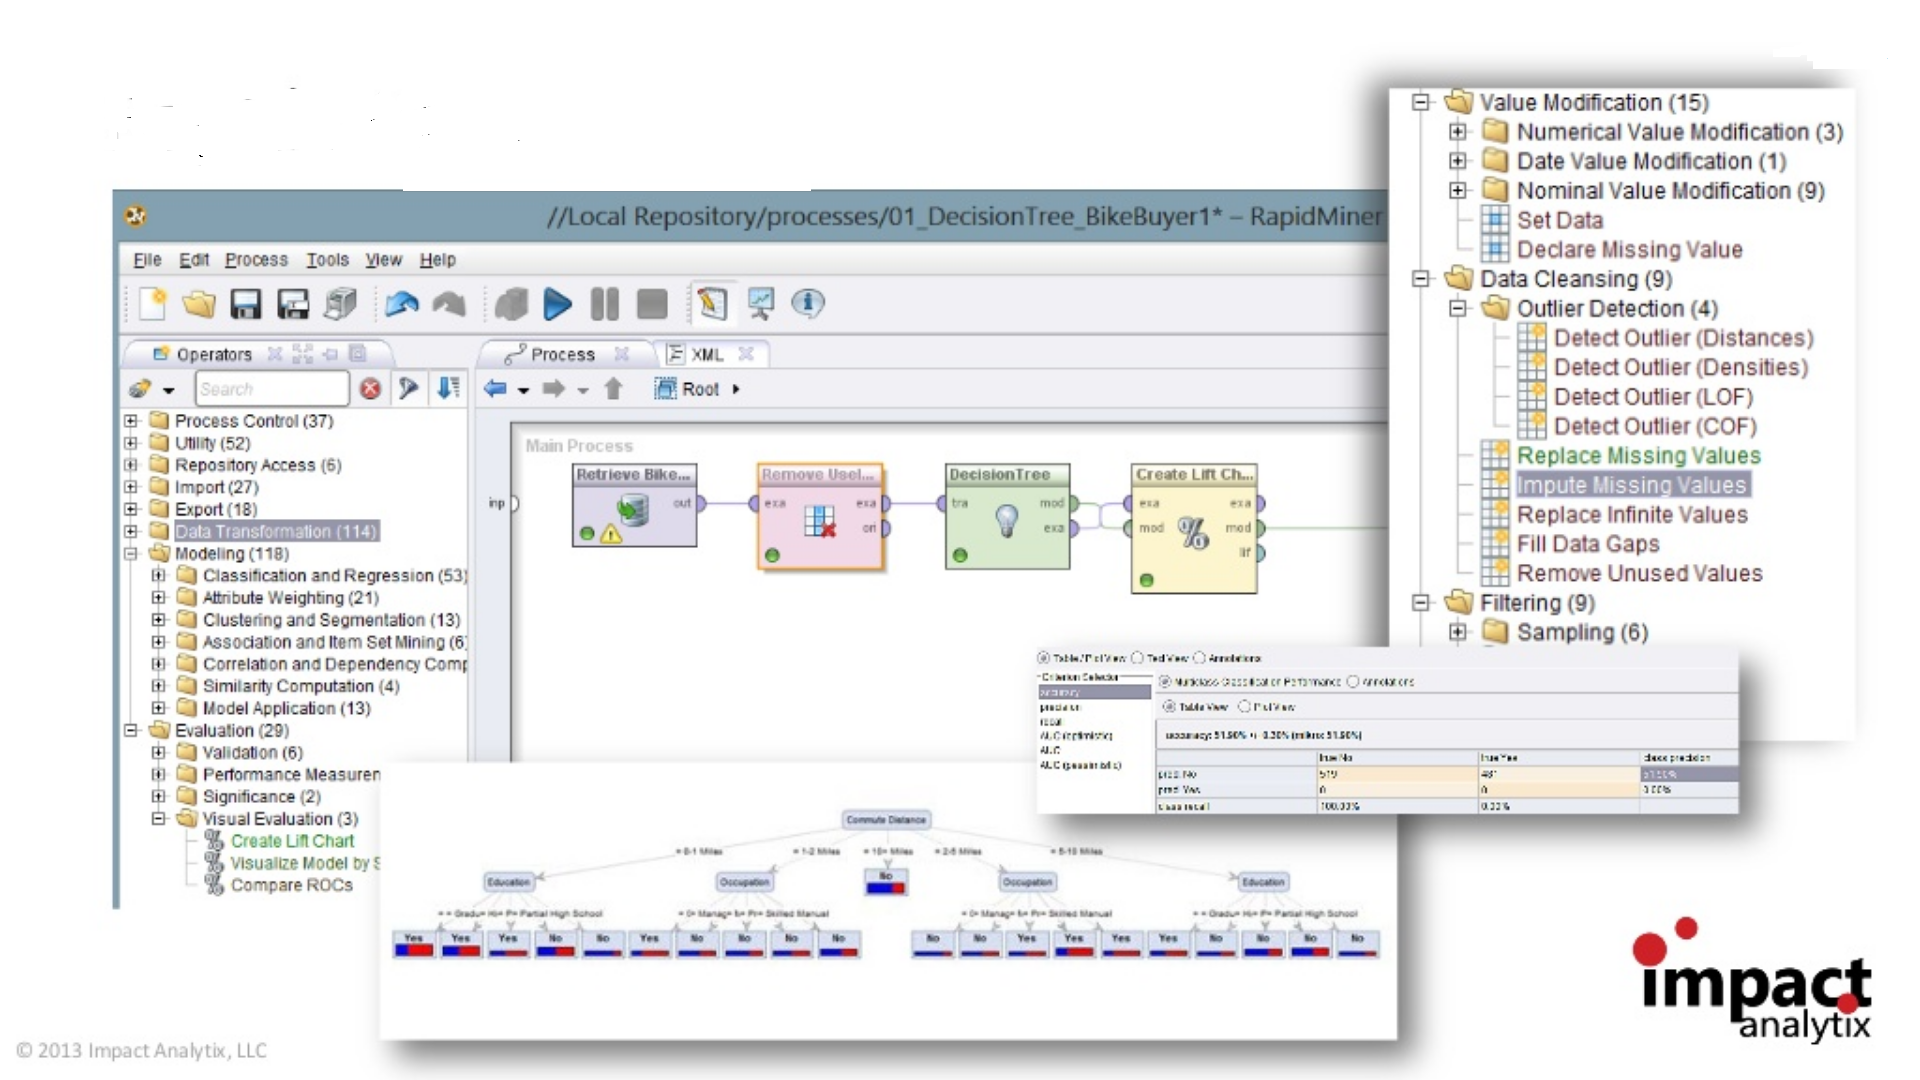
\includegraphics[width=\linewidth]{predanat8}
\end{center}

{\tiny (Ref: Practical Predictive Analytics - Jen Underwood )}


\end{frame}

%%%%%%%%%%%%%%%%%%%%%%%%%%%%%%%%%%%%%%%%%%%%%%%%%%%%%%%%%%%%%%%%%%%%%%%%%%%%%%%%%%
\begin{frame}\frametitle{R and Rattle}

\begin{center}
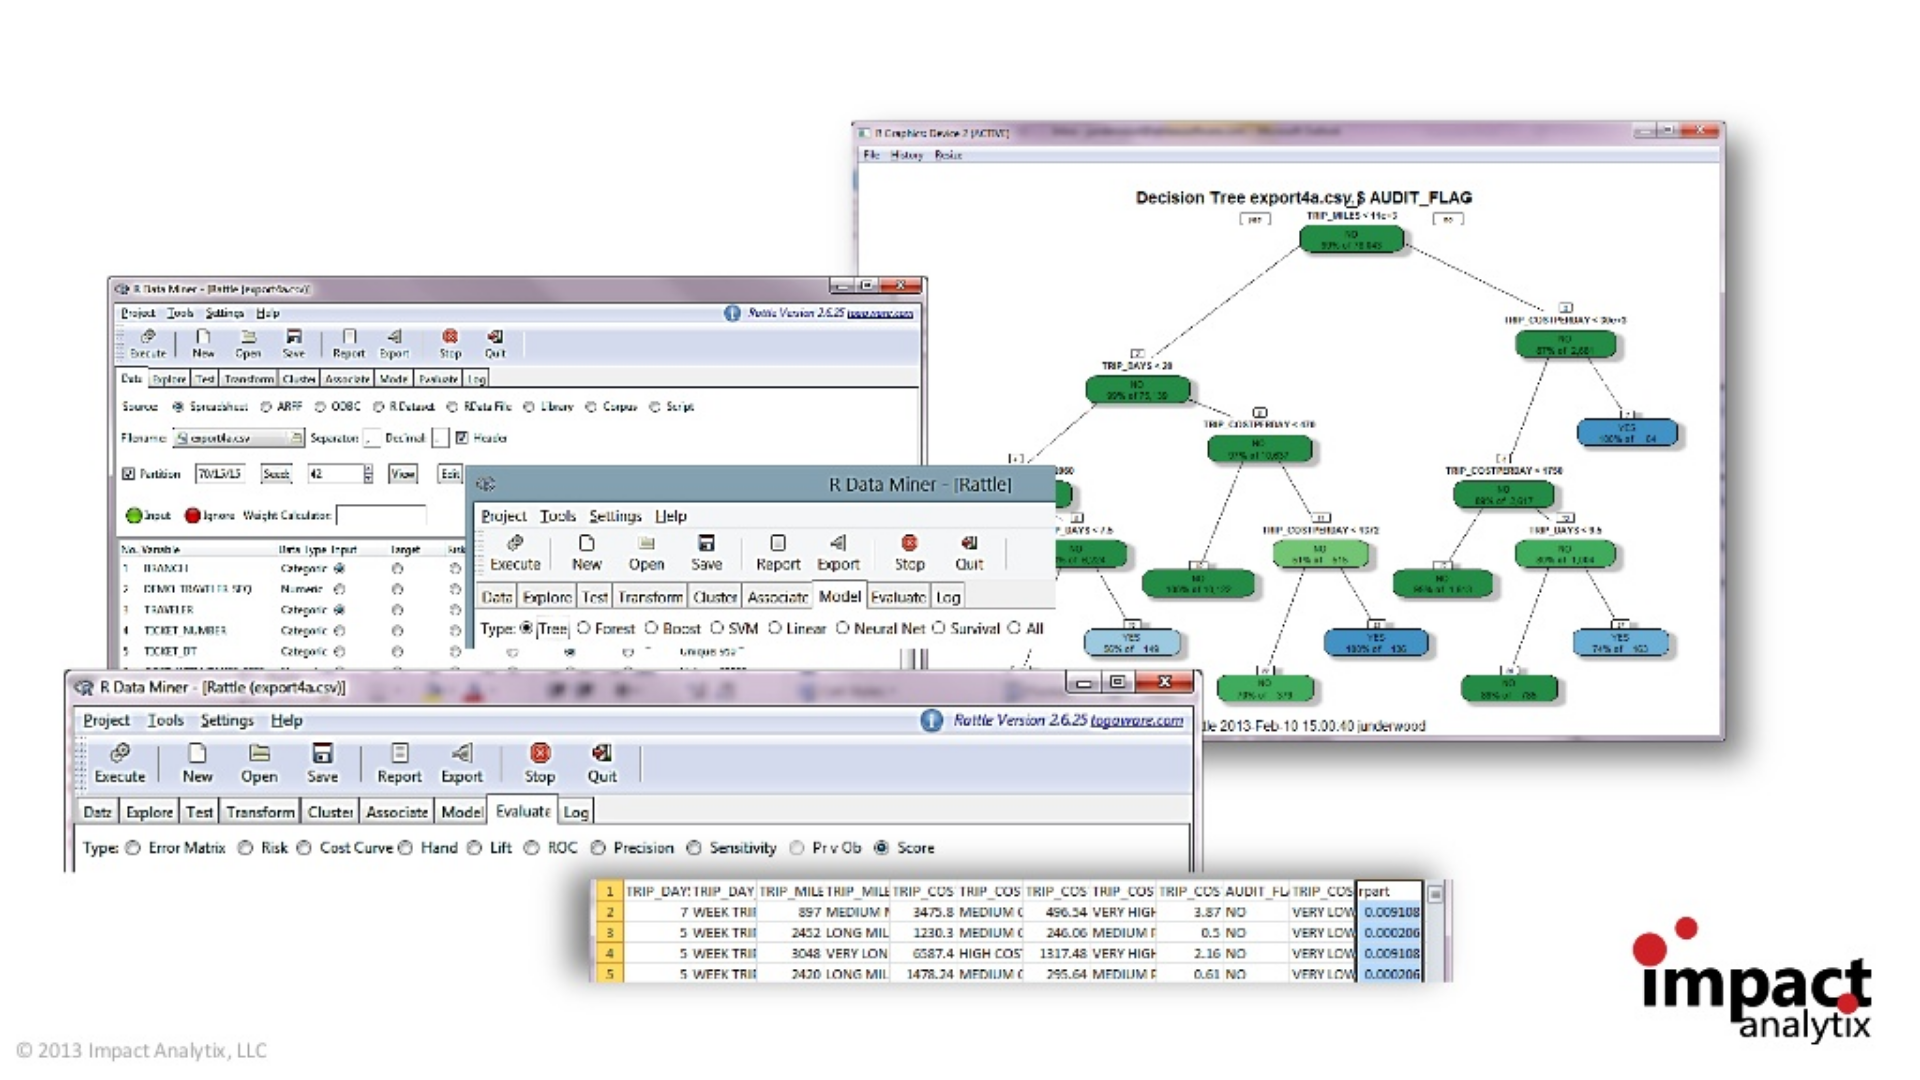
\includegraphics[width=\linewidth]{predanat9}
\end{center}

{\tiny (Ref: Practical Predictive Analytics - Jen Underwood )}


\end{frame}

%%%%%%%%%%%%%%%%%%%%%%%%%%%%%%%%%%%%%%%%%%%%%%%%%%%%%%%%%%%%%%%%%%%%%%%%%%%%%%%%%%
\begin{frame}\frametitle{Microsoft Excel}

\begin{center}
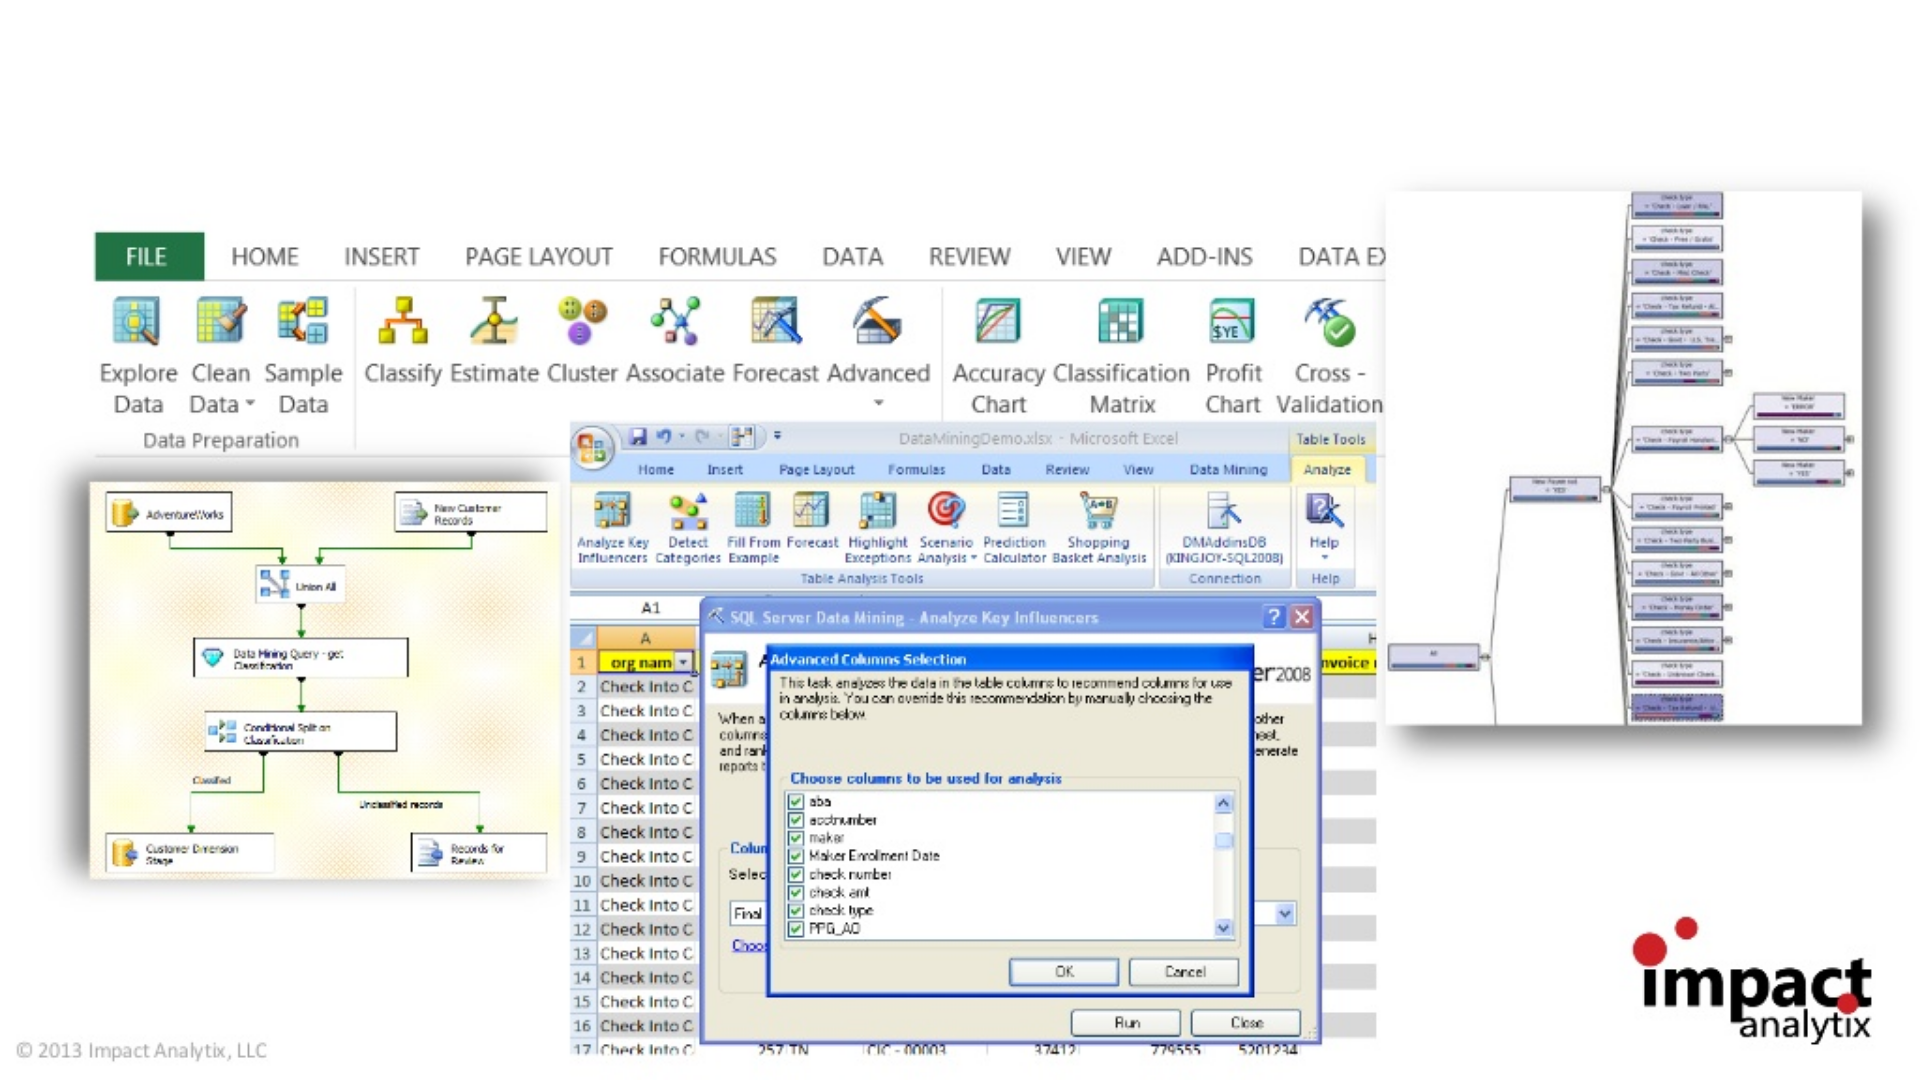
\includegraphics[width=\linewidth]{predanat10}
\end{center}

{\tiny (Ref: Practical Predictive Analytics - Jen Underwood )}


\end{frame}

%%%%%%%%%%%%%%%%%%%%%%%%%%%%%%%%%%%%%%%%%%%%%%%%%%%%%%%%%%%%%%%%%%%%%%%%%%%%%%%%%%
\begin{frame}\frametitle{Pentaho Weka}

\begin{center}
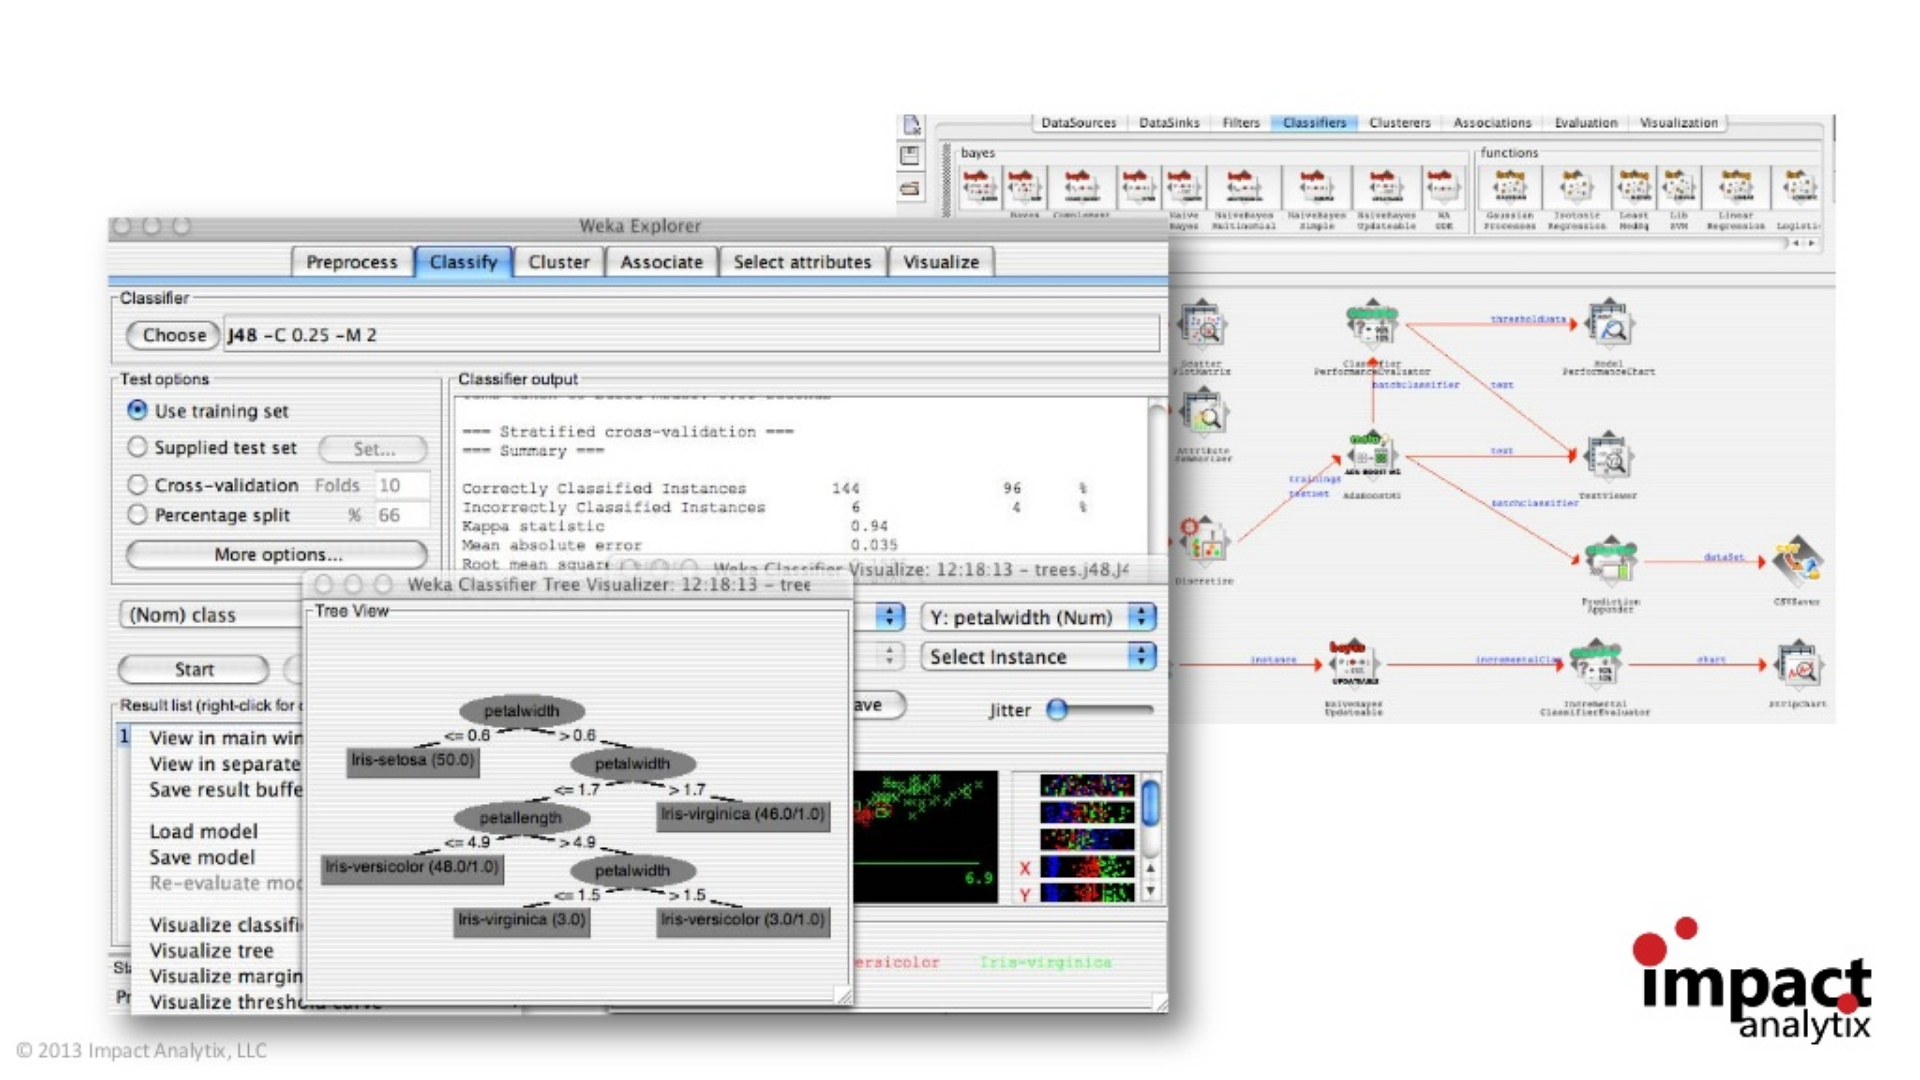
\includegraphics[width=\linewidth]{predanat11}
\end{center}

{\tiny (Ref: Practical Predictive Analytics - Jen Underwood )}


\end{frame}

%%%%%%%%%%%%%%%%%%%%%%%%%%%%%%%%%%%%%%%%%%%%%%%%%%%%%%%%%%%%%%%%%%%%%%%%%%%%%%%%%%
\begin{frame}\frametitle{SAS Enterprise Miner}

\begin{center}
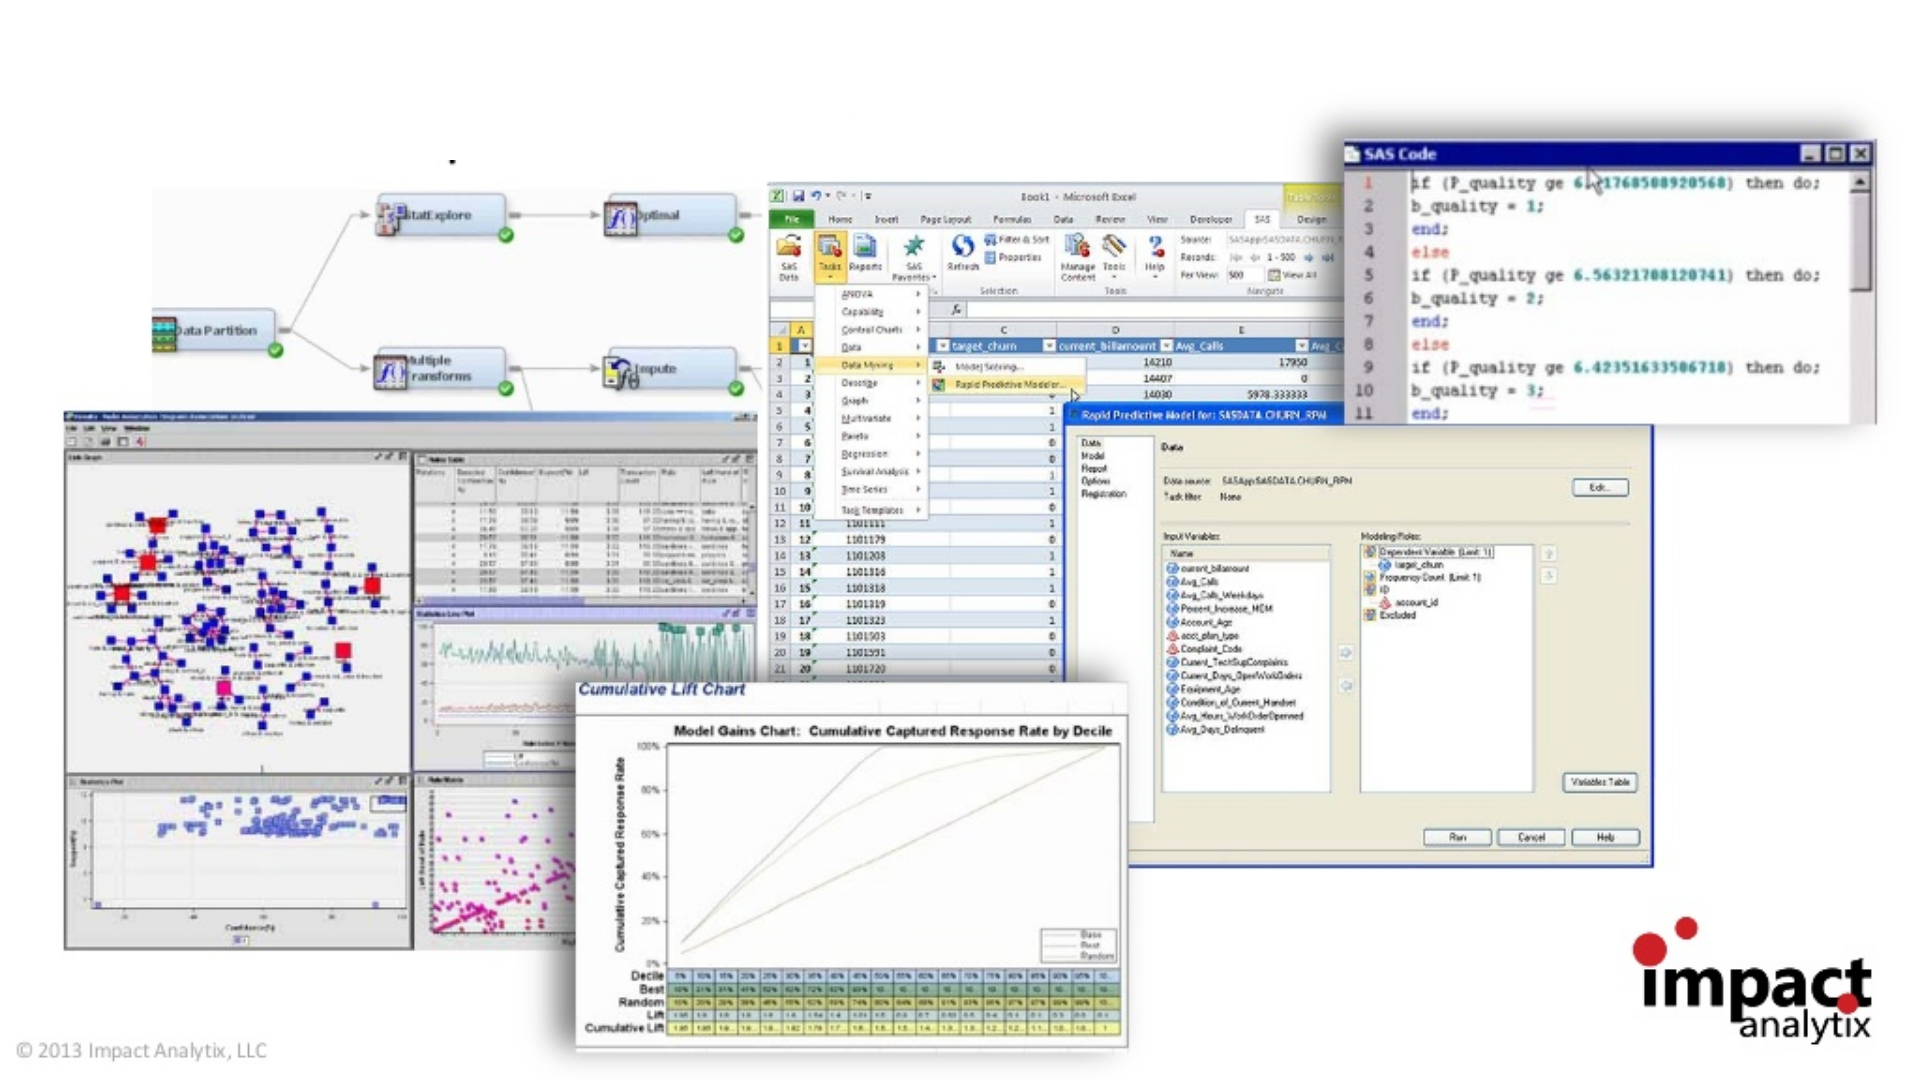
\includegraphics[width=\linewidth]{predanat12}
\end{center}

{\tiny (Ref: Practical Predictive Analytics - Jen Underwood )}


\end{frame}

%%%%%%%%%%%%%%%%%%%%%%%%%%%%%%%%%%%%%%%%%%%%%%%%%%%%%%%%%%%%%%%%%%%%%%%%%%%%%%%%%%
\begin{frame}\frametitle{IBM SPSS Modeler}

\begin{center}
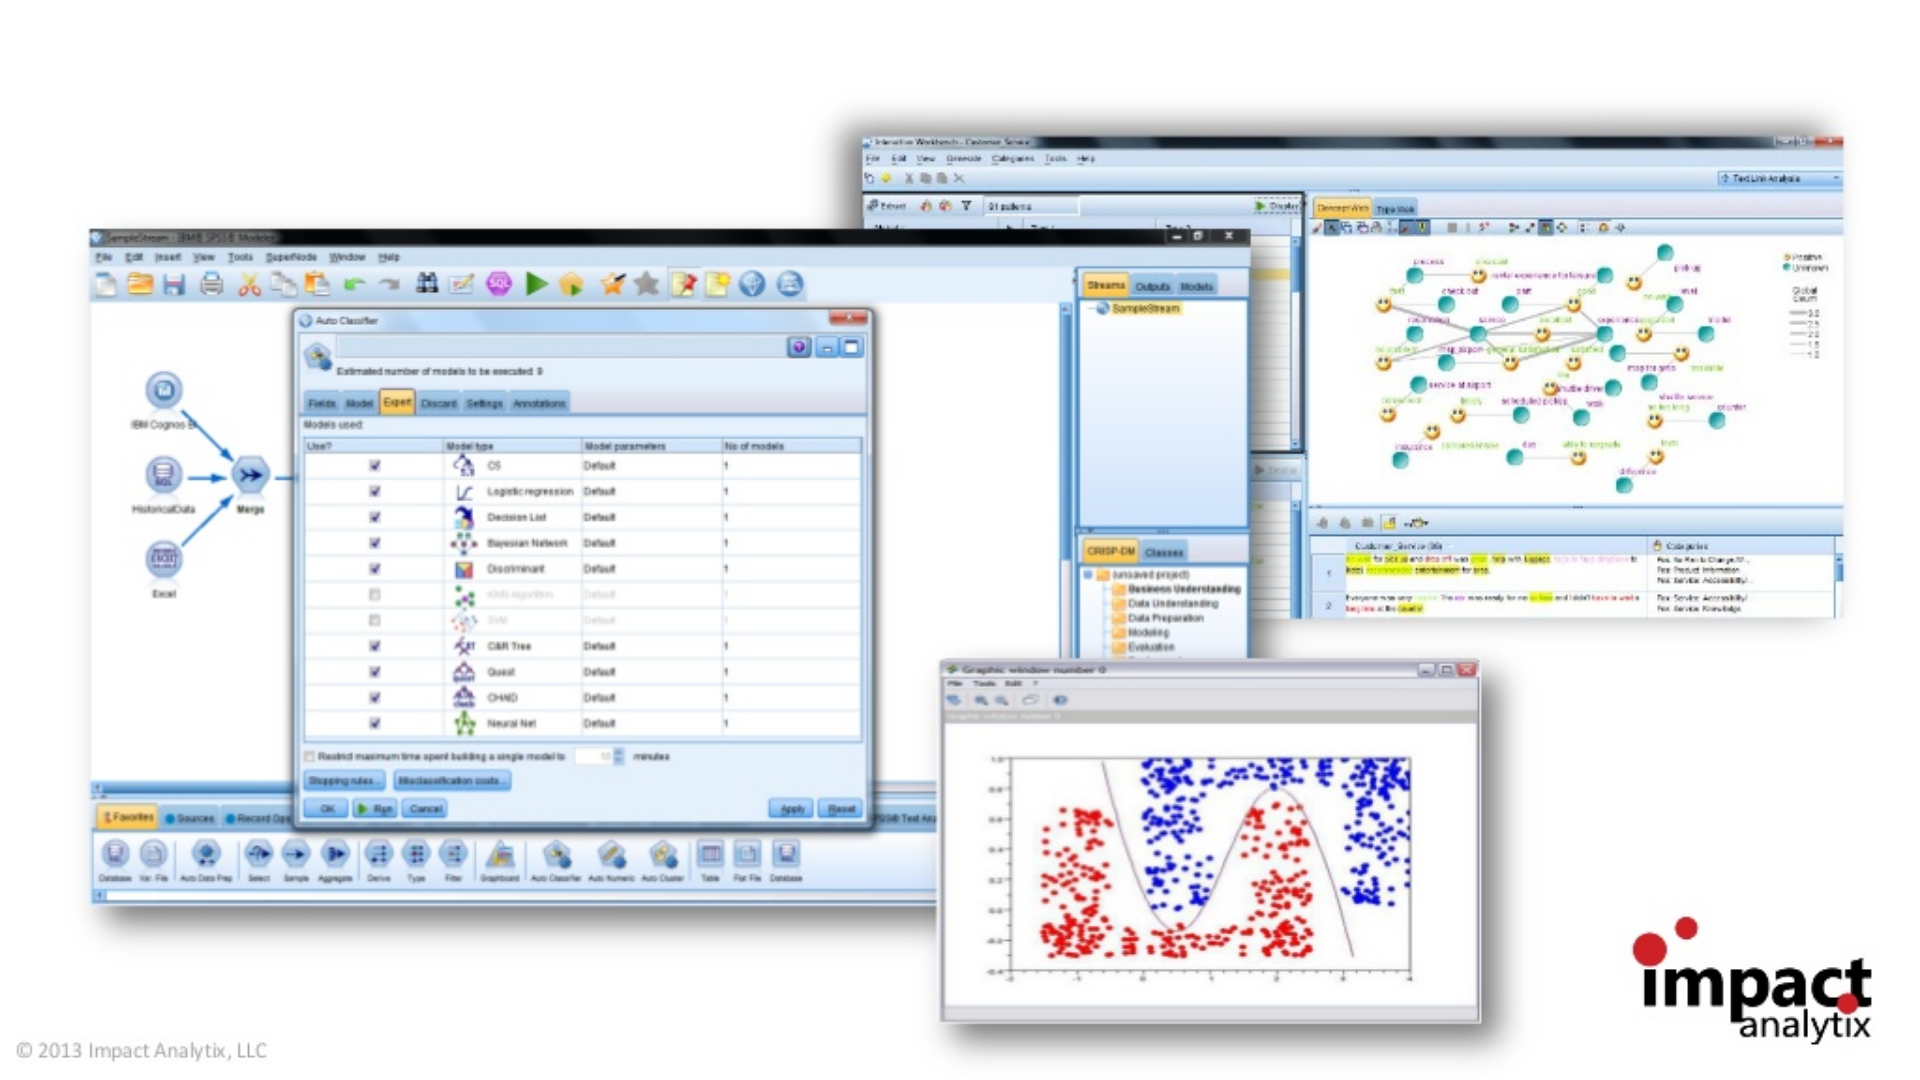
\includegraphics[width=\linewidth]{predanat13}
\end{center}

{\tiny (Ref: Practical Predictive Analytics - Jen Underwood )}


\end{frame}

%%%%%%%%%%%%%%%%%%%%%%%%%%%%%%%%%%%%%%%%%%%%%%%%%%%%%%%%%%%%%%%%%%%%%%%%%%%%%%%%%%
\begin{frame}\frametitle{Oracle Data Miner}

\begin{center}
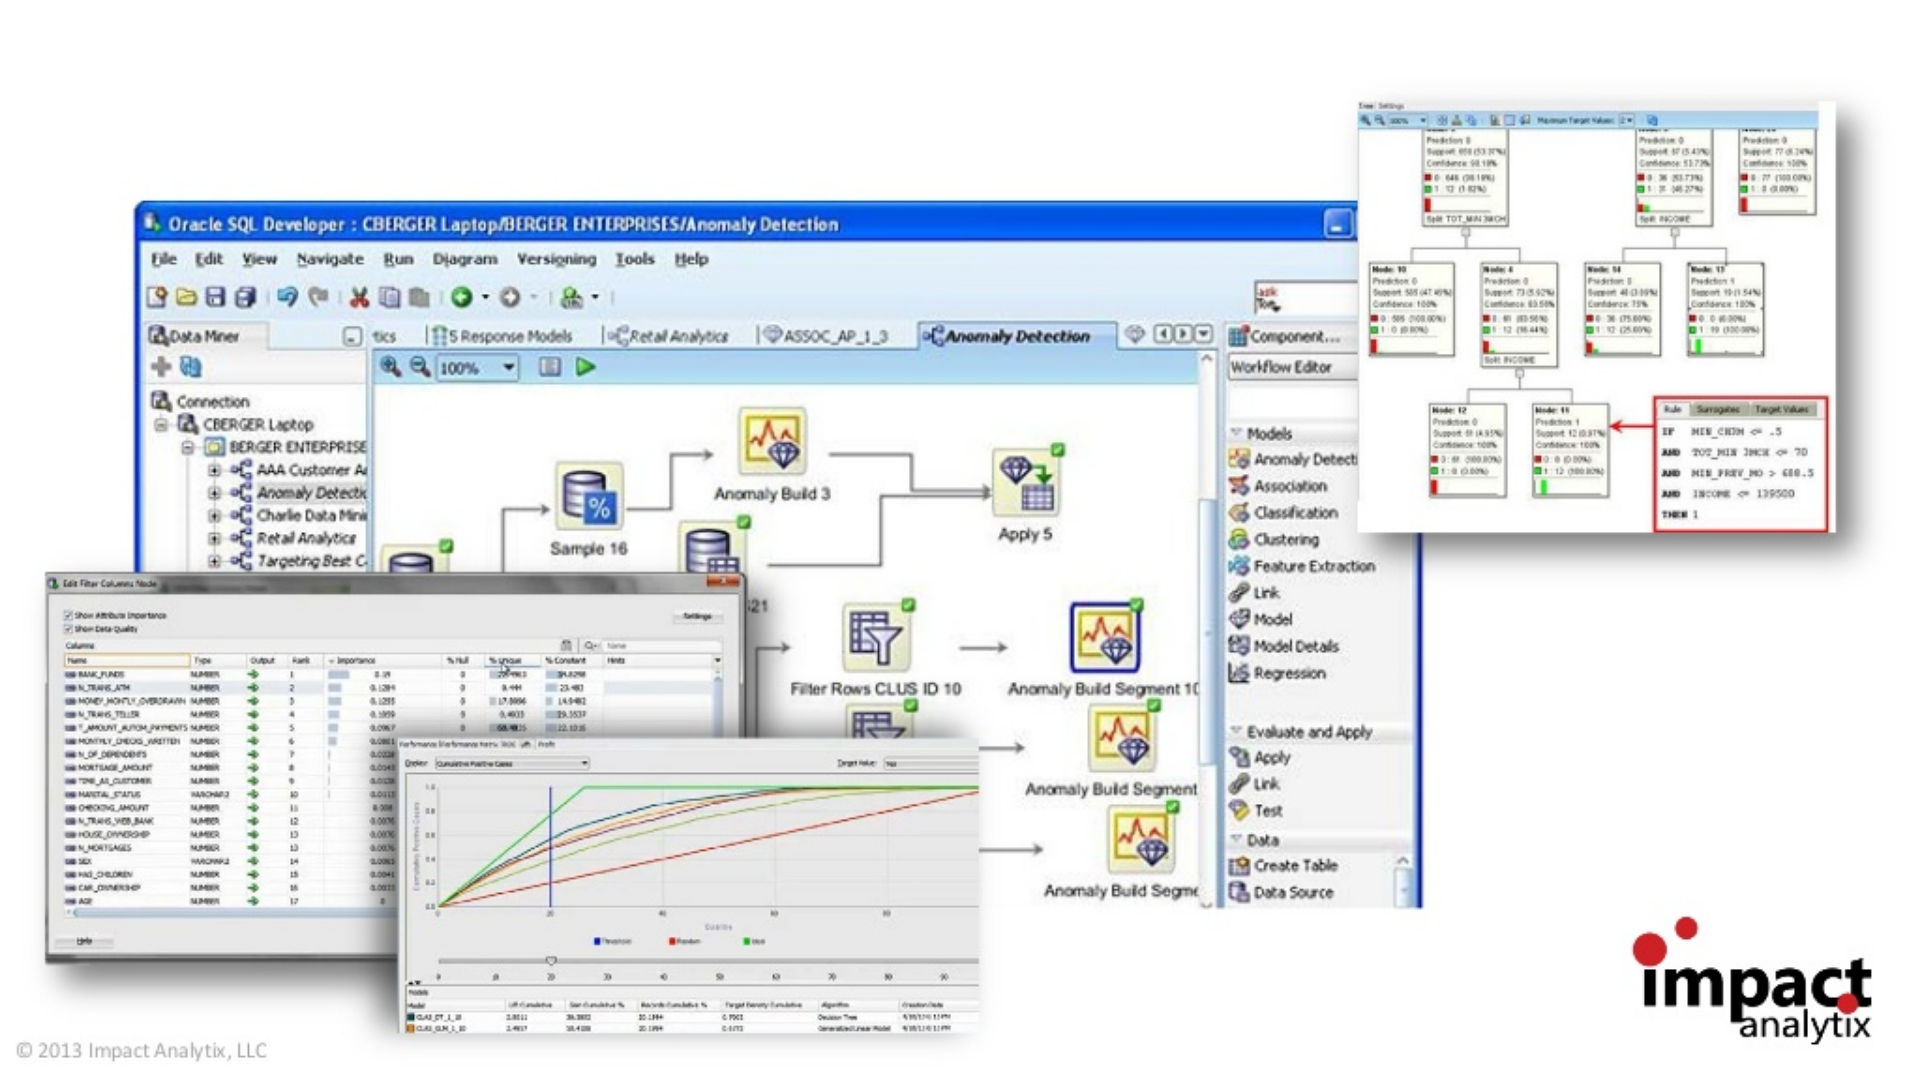
\includegraphics[width=\linewidth]{predanat14}
\end{center}

{\tiny (Ref: Practical Predictive Analytics - Jen Underwood )}


\end{frame}

%%%%%%%%%%%%%%%%%%%%%%%%%%%%%%%%%%%%%%%%%%%%%%%%%%%%%%%%%%%%%%%%%%%%%%%%%%%%%%%%%%
\begin{frame}\frametitle{Tableau}

\begin{center}
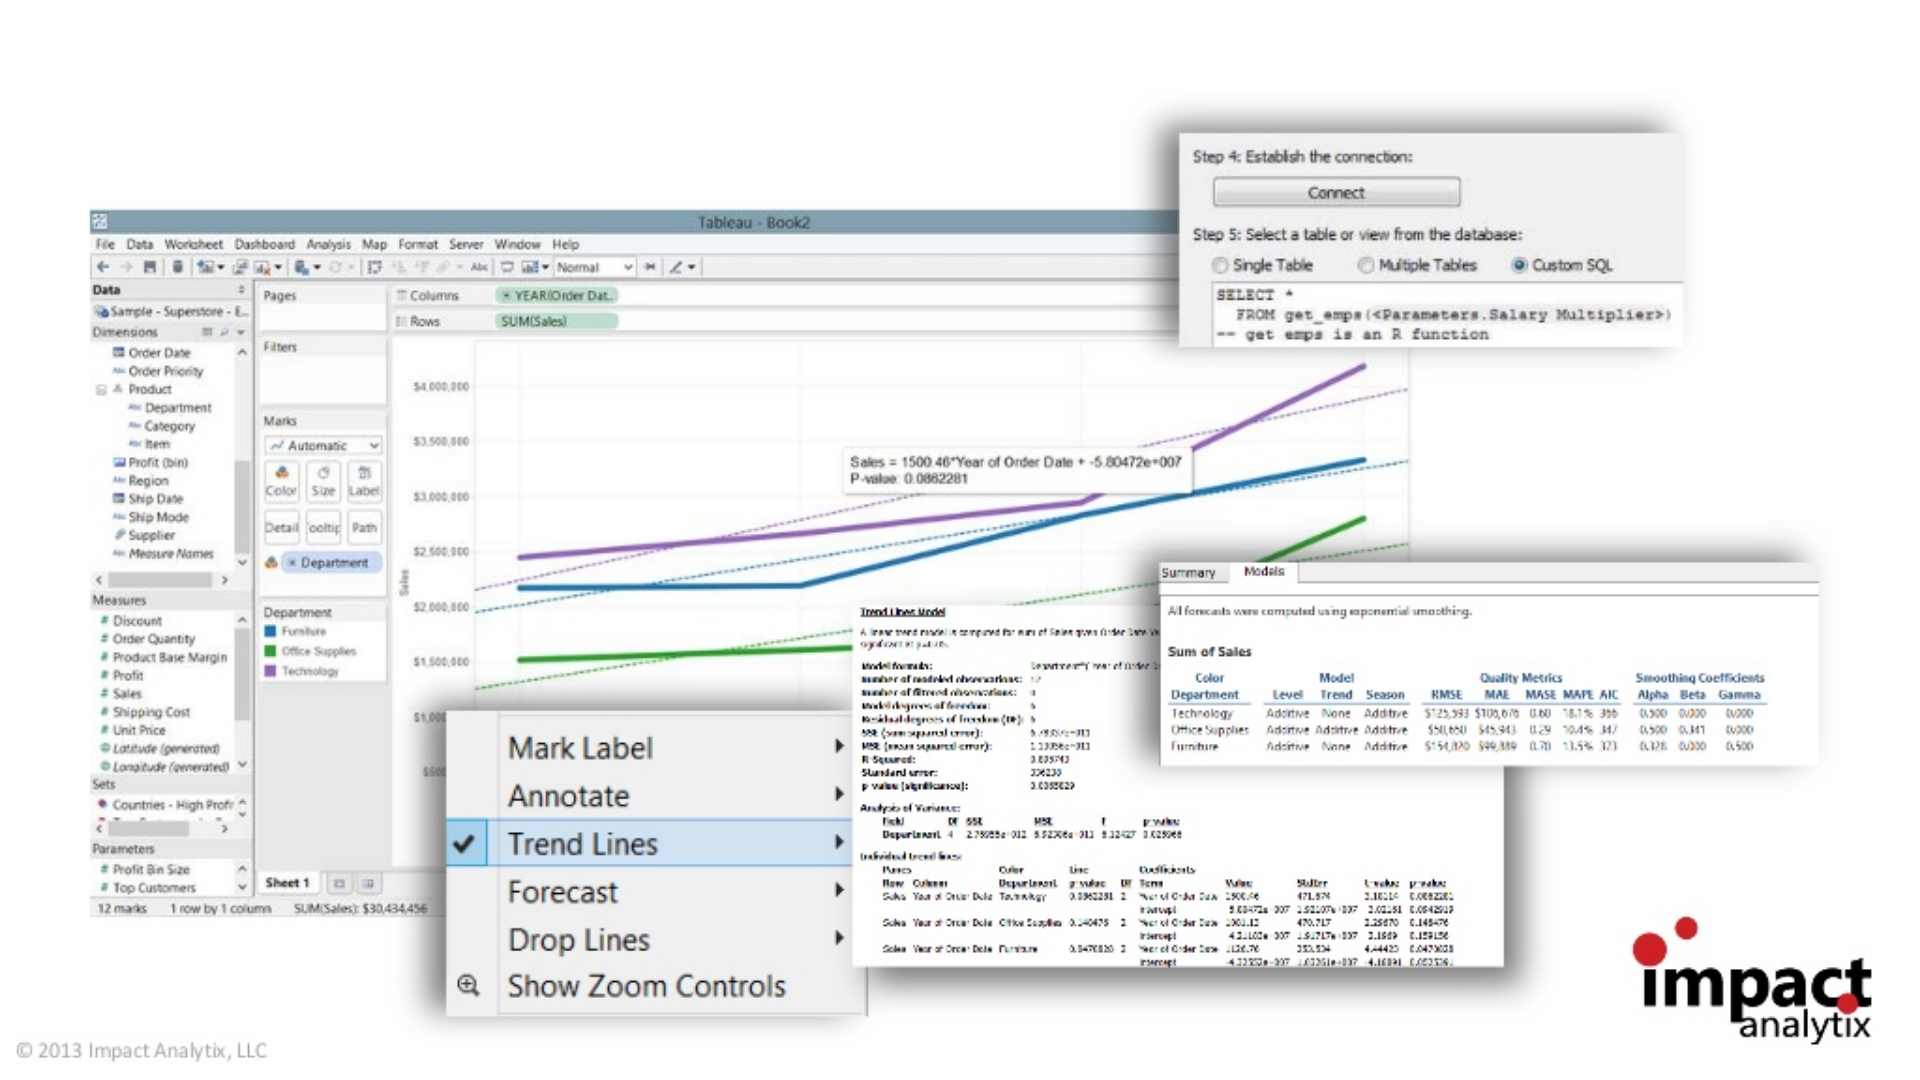
\includegraphics[width=\linewidth]{predanat15}
\end{center}

{\tiny (Ref: Practical Predictive Analytics - Jen Underwood )}


\end{frame}

%%%%%%%%%%%%%%%%%%%%%%%%%%%%%%%%%%%%%%%%%%%%%%%%%%%%%%%%%%%%%%%%%%%%%%%%%%%%%%%%%%
\begin{frame}\frametitle{Next?}
Learn Machine Learning!!!
\begin{itemize}
\item ``The powerhouse organizations of the Internet era, which include Google and
Amazon \ldots have business models that hinge on predictive models based on machine
learning.''

- Professor Vasant Dhar, Stern School of Business, New York University

\item ``A breakthrough in machine learning would be worth 10 Microsofts.'' 

- Bill Gates
\end{itemize}

\end{frame}

